\chapter{Description and Evaluation of Current Work}
\section{Introduction}
The work has completed up to this stage including composing the ethics proposal for data collection and developing a system on a cloud platform for the feasibility test on the mock dataset created for temporary use. The experiment consisting of two series were introduced in the ethics proposal as the guideline for data collection in next phase. Initial experimenting work on exploring potential signal processing combinations, useful features and classifiers has been carried out. The tools, approaches applied and results obtained for the current stage are shown and evaluated in this chapter.

\section{System architecture}
The system architecture consisted of three major parts as shown in Fig. \ref{fig:system_architecture}. Data preparation and pre-processing were included in the first part. The pre-processed data was then passed to the second part of the system for feature extraction to obtain the essence of the signal. The last part of the system was responsible for two jobs, classification and estimation. The classifier discriminated segmentations based on the feature extracted and then estimated respiration related information such as respiratory frequency, respiratory phase, and respiratory depth. 

\begin{figure}[h]
    \centerline{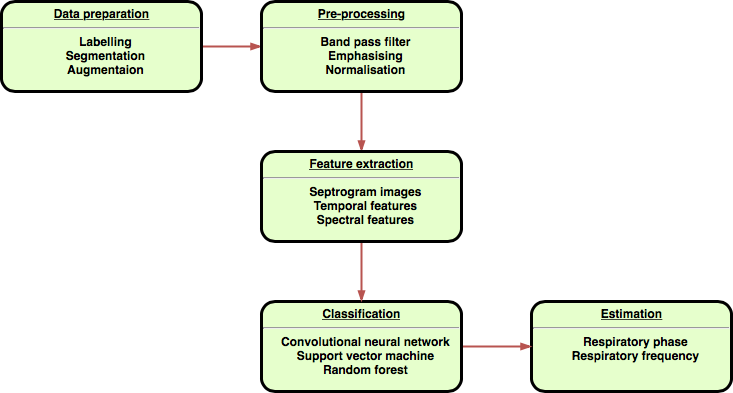
\includegraphics[scale=0.55]{figures/system_architecture.png}}
    \caption{A diagram of the system architecture}
    \label{fig:system_architecture}
\end{figure}

\section{Environment setup}
Instead of developing the system directly for the mobile platform at the initial stage, the experiment was carried out on Colaboratory. Colaboratory is an cloud Jupyter Notebook environment and ideally for fast-prototyping. The experiment programs are written in Python which is widely used in machine learning and deep learning community. Test data was stored on Google drive which is then connected to the Jupyter notebook created on Colaboratory. This approach made the file importing and exporting effortless and reliable in the experimenting process. 

There were also a number of Python libraries considered in this experiment for various purposes. Librosa is a Python library focused on audio signal processing, it implements most of the popular signal processing approaches and enables easy access to the frequently-used features in temporal and spectral analysis. PyHHT and PyWT were also tested for the implementation of Hilbert Huang Transform and Wavelet Transform, respectively. Matplotlib was selected to achieve visualisation and plots exporting. 

\section{Dataset preparation}
Prior to receiving the approval for the ethics application, a mock dataset was temporarily created from the author during a short running outdoors. The mock dataset consisted of 4 audio files in WAV format which were recorded in 22050Hz with the iOS application named Audio Memos using IPhone 6 and the microphone in the original earpods. The duration of the audio clips varies from 23 to 59 seconds.

The exhalation and inspiration segmentation contained in the dataset were manually labelled.An example of the test data with respiration phase labels is illustrated in Fig. \ref{fig:audio_waveform}. However, the markers in yellow and red only represent when the inhalation and exhalation approximately begin. A more precised and completed labelling could be obtained after the actual data collection.

\begin{figure}[h]
    \centerline{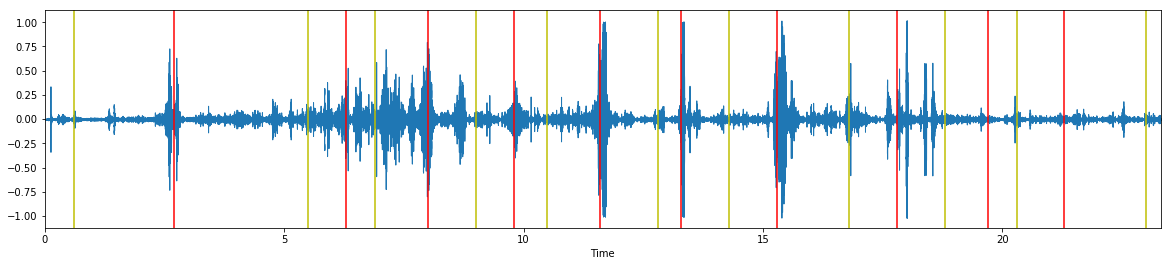
\includegraphics[scale=0.35]{figures/audio_waveform.png}}
    \caption{An illustration of a respiratory sound signal with manual labelling. Inhalation starts at yellow markers. Exhalation starts at red markers.}
    \label{fig:audio_waveform}
\end{figure}

\clearpage
\section{Signal processing methods}
The complete pre-processing pipeline consisted of 4 steps which were a band-pass filter, an emphasis filtering, normalisation and segmentation. The design of the combination of signal processing methods were inspired by \cite{Lei2014Content-basedFeatures}\cite{Niu2019AState}\cite{Ren2015Fine-grainedSmartphones}. The completed results after applying the full pre-processing techniques is shown in Fig. \ref{fig:fft_pipeline}.
\begin{figure}[h]
    \centerline{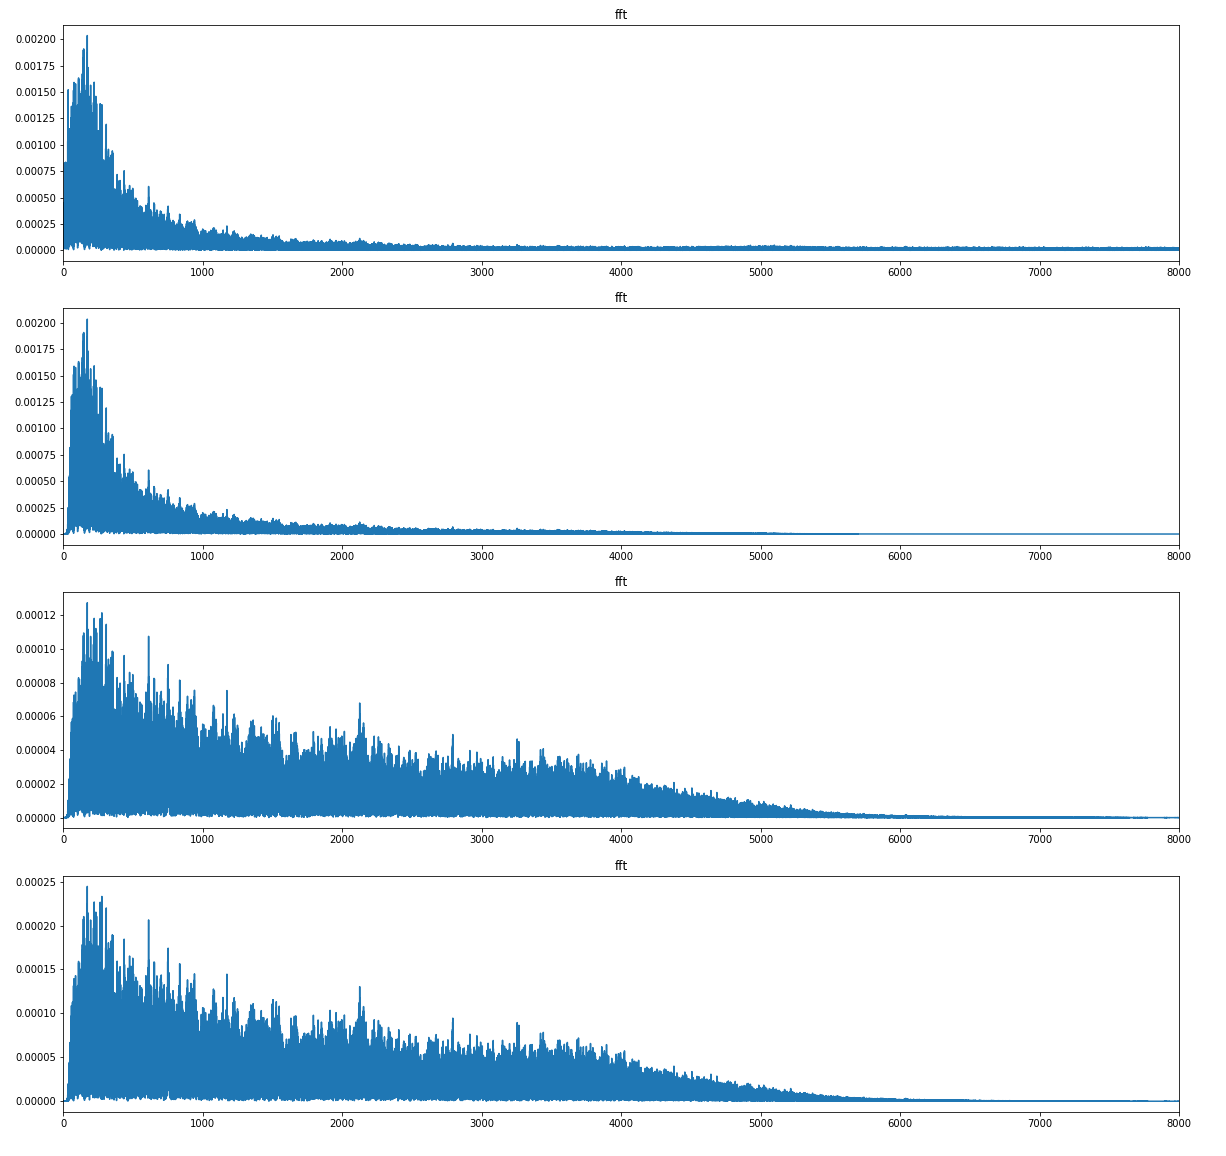
\includegraphics[scale=0.33]{figures/fft_pipeline.png}}
    \caption{The results of applying the complete signal processing methods.}
    \label{fig:fft_pipeline}
\end{figure}

\subsection{Band-pass filter}
The frequency components that contained in the four audio clips were  examined by applying Fast Fourier Transform (FFT) as shown in Fig. \ref{fig:fft}. It was clearly shown that the major frequency components were in the range of 0-2000Hz. To filter out the rest unwanted frequency, the signal data was firstly fed into a band-pass filter to retain the frequency component between 50Hz and 4000Hz. 

\begin{figure}[h]
    \centerline{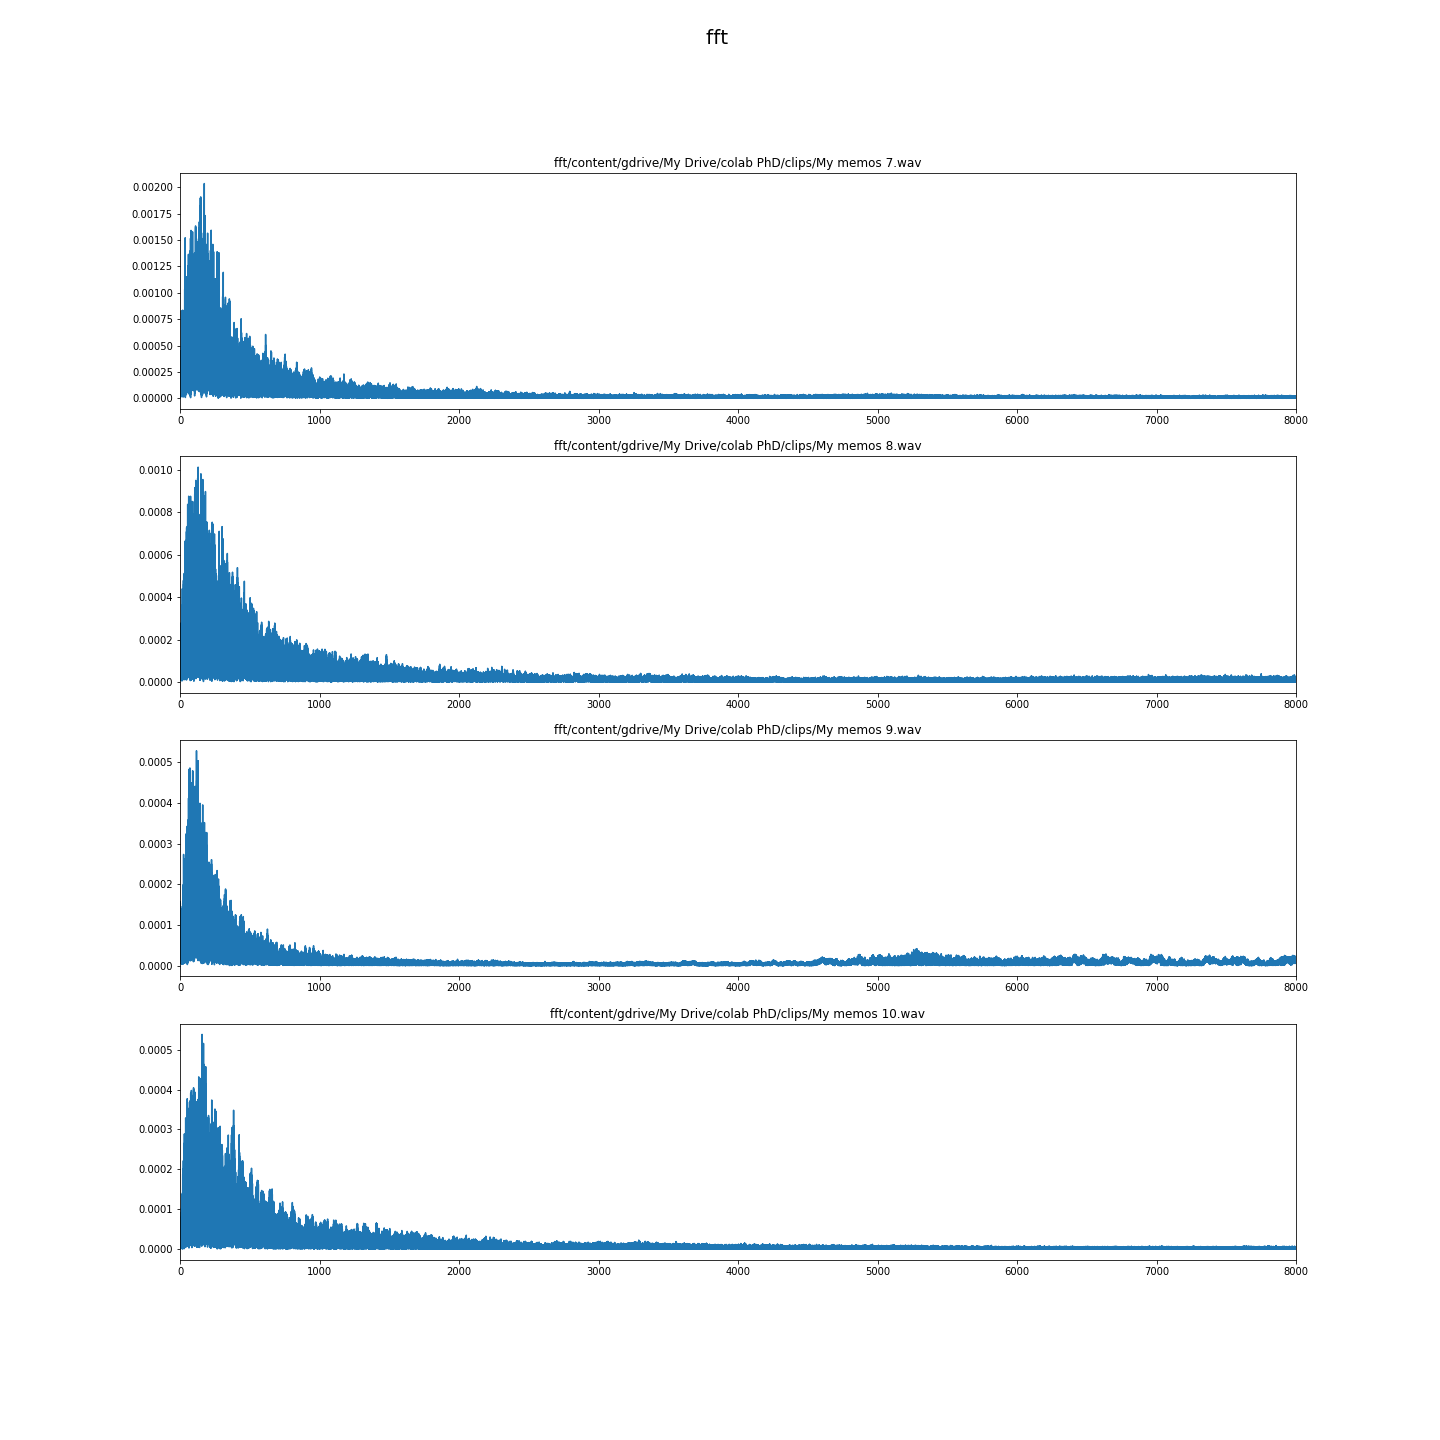
\includegraphics[scale=0.33]{figures/fft.png}}
    \caption{Frequency components of four respiratory sound signals decomposed using FFT}
    \label{fig:fft}
\end{figure}

\subsection{Emphasis filter}
To overcome the radiation effects caused mostly by the lips, the signals were applied with a pre-emphasised filter to increase the amplitude of the frequency components in high frequency range. This step is achieved by following 
\begin{equation}
s^\prime (i)=s(i) - 0.96 \times s(i-1), \qquad i=1, \ldots, N-1
\end{equation}
where $s(i)$ is the i-th sample data in the signal and $s^\prime(0) = s(0)$ when $i=0$.

\subsection{Normalisation}
Due to the variations of the devices used and the location the signals collected from, it is suggested to normalise the signal to have a stable performance.
\begin{equation}
s^\prime (i)=\frac{s(i)}{\max(|s(i)|)}
\end{equation}

\subsection{Segmentation}
Segmentations are 1000ms long having 22050 signal data points and 25\% overlapping. Hamming window is applied to segmentations to avoid spectral leakage effect. It is worth noting that segmentations created for training were likely to include some of the non-respiration sound because of the subjective labelling. Therefore, it should affect the performance of the classifier described below. 

\section{Feature extraction}
This research aims to explore the most suitable representation of spectrograms and spectral and temporal features. The results of feature extraction obtained are evaluated in the following sections. 

\subsection{Spectral features}
As illustrated in last section, FFT is great for decomposing the frequency components included in the signals. However, it only demonstrate very little information regarding the relationship between time and frequency. In order to extract the correlation between time and frequency in the signal, a number of frequency domain-based analysing approaches were evaluated, such as Short Time Fourier Transform (STFT), Wavelet Transform (WT) and Hilbert Huang Transform (HHT).

STFT provides time-frequency information by applying FFT on the window with fixed length sliding across entire signals. The spectrograms generated by STFT is then converted to mel-scaled spectrograms. Mel-scale is more ideal for representing human sound in frequency due to the fact that the non-linear perception of humans' hearing to different frequency. The comparison between STFT generated spectrogram and its mel-scaled spectrogram is shown in Figure \ref{fig:stft_mel-stft}. The mel-scaled spectrogram provides a more intuitive visualisation for exhalation than the original spectrogram. It clearly shows that most of the red markers perfectly align with one of the peaks in the spectrogram. The red markers which do not associate with any peaks were also hard to distinguish during labelling. On the other hand, it is relatively impossible to recognise the inhalation by simply looking at the mel-scaled spectrogram. 

\begin{figure}[h]
    \centerline{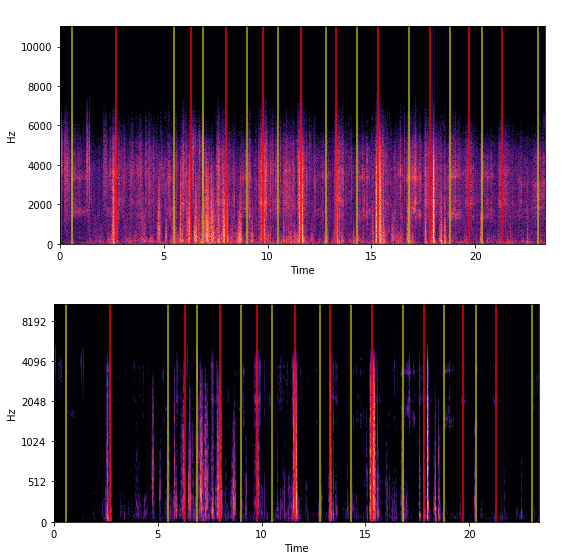
\includegraphics[scale=0.55]{figures/stft_mel-stft.png}}
    \caption{The spectrograms obtained from using STFT (top plot) and mel-scaled STFT (bottom plot). Inhalation starts at yellow markers. Exhalation starts at red markers.}
    \label{fig:stft_mel-stft}
\end{figure}

STFT has same resolution across different frequency range which is not a ideal approach for non-stationary signals with fast transient features. In contrast, WT offers good resolution in time and relatively weak resolution in frequency in high frequency range while good resolution in frequency and relatively weak resolution time in low frequency range. It would be helpful to capture the transients features by adopting continuous wavelet transform. Different wavelet functions influences the results of spectrogram generated. There were three kinds (Gaus, Mexh and Morl) of continuous wavelet function experimented as the basis functionand the results are shown in Fig. \ref{fig:wavelet_functions}. It is fairly difficult to identify which wavelet function gives the best results in representing the signal.

\begin{figure}[h]
    \centerline{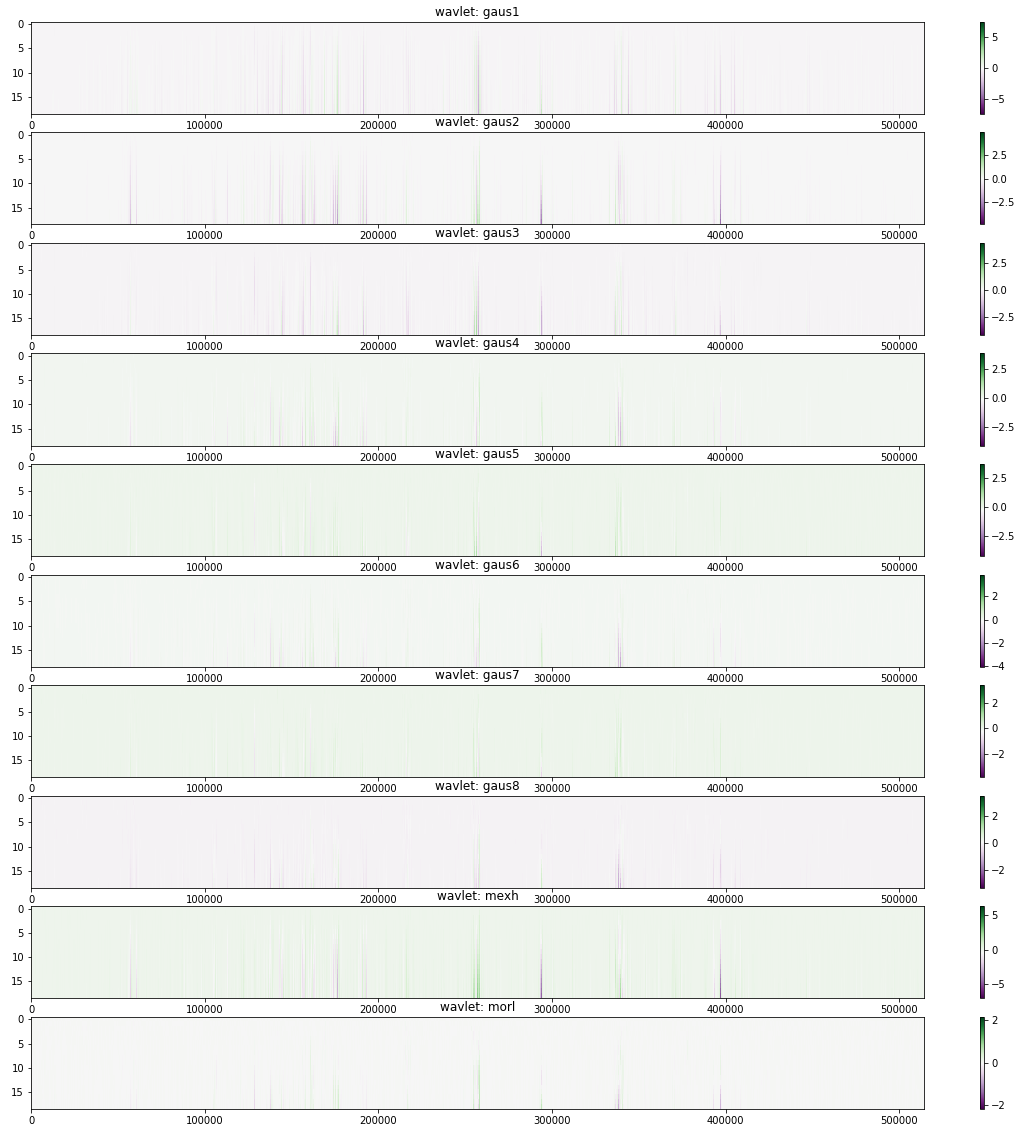
\includegraphics[scale=0.45]{figures/wavelet_trans_wav_func.png}}
    \caption{The result of applying different wavelet functions to a respiratory sound signal}
    \label{fig:wavelet_functions}
\end{figure}

\clearpage
\subsection{Temporal features}
The energy of an individual segmentation is the only temporal feature which has been implemented and evaluated so far. The energy of a segmentation is define as 
\begin{equation}
e(i) = \sum_{i=0}^{N-1}{s(i)^2}
\end{equation}

where N is the size of a segmentation and $s(i)$ is the i-th data point in a segmentation.

The purpose of using energy is to discriminate voiced and unvoiced segmentations. It could significantly reduce time spent in computation by disregarding the unvoiced segmentation in classification. This audio signal is 23s long containing 2678 segmentations as shown in Fig. \ref{fig:energy}. By setting energy threshold to the mean of the energy across the signals, only 309 segmentations were retained which still include around 90\% of the inhalation and exhalation segmentations. Therefore, segmentation energy is an effective feature in screening voiced and unvoiced segmentation. 

\begin{figure}[h]
    \centerline{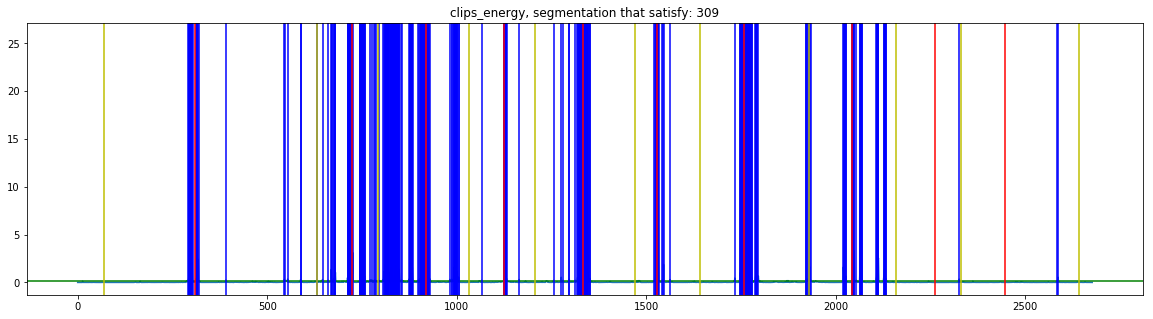
\includegraphics[scale=0.35]{figures/energy.png}}
    \caption{The blue line on the top plot represents the segmentation energy for all segmentations of a respiratory sound signal. The navy colour markers on the bottom plot correspond to the segmentations having higher energy than the energy threshold.}
    \label{fig:energy}
\end{figure}

\section{Data representation}
In order to generate training data for CNN, the spectrograms of the signals which represent inhalation and exhalation will be generated and saved in corresponding folders on the Google drive for easy access from Colaboratory. In total, there were 51 inhalation segmentations and 54 exhalation segmentations created from four respiration sound files. 20\% of the segmentation were randomly selected and then used as valid data. Partial mock dataset is shown in Fig. \ref{fig:dataset}

\begin{figure}[h]
    \centerline{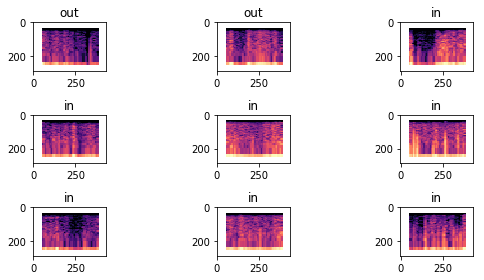
\includegraphics[scale=0.8]{figures/dataset.png}}
    \caption{Partial dataset (Spectrograms titled as 'in' represents an inhalation data. Spectrograms titled as 'out' represents an exhalation data.}
    \label{fig:dataset}
\end{figure}

\section{Classification}
Being able to correctly discriminate the sound of inhalation and exhalation is the foundation of providing respiration-related information such respiratory phase and depth. To quickly explore the feasibility of classifying respiration sound using audio signal generated spectrograms, FastAI was selected for implementation. FastAI is a high-level deep learning framework enables fast and easy process in deep learning model training and analysing. 

Transfer learning allows taking advantage of past experience from previous training. FastAI provides pre-trained models for transfer learning without developing and training a neural network from scratch. ResNet34 is a variation of convolutional neural network was used in this phase \cite{He2016DeepRecognition}.

The performance of the training phase was evaluated through three characteristics training loss, valid loss and accuracy. The model was trained for 10 epochs and the final accuracy achieved over the validation dataset was 66\%. Even the loss on the training dataset decreased over the epochs but it was significantly higher than the loss on the validation dataset. It was likely to be a sign of underfitting which suggested that the model didn't learn enough characteristics for classification from the mock dataset prepared. It might also imply that the classification model is not ideal for respiration data. However, the classification results were obtained without fine-tuning. Approaches used to improve classifier's performance is described in the next chapter. 
\begin{figure}[h]
    \centering
    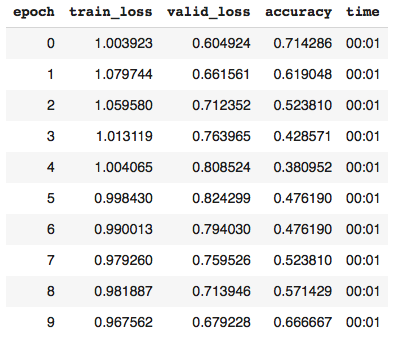
\includegraphics[scale=0.6]{figures/classification_results.png}
    \caption{Results after ten epochs training.}
    \label{fig:classification_results}
\end{figure}